\section{Feature Engineering}\label{sec:feature_eng}
In this section, we will elaborate on the feature engineering for the experiments. Feature engineering concerns extracting useful features from the dataset.  %The idea behind data pipeline is to automate the workflow for training and testing a model. A data pipeline consists of a sequence of data processing components, where the output of one component would be the input to another. For the position estimation in this project, we need a data pipeline to model the different scene analysis algorithms and evaluate them as well as the \gls{imu}-based algorithms. The responsibility of the data pipeline to process the data from the preprocessing step to a format directly usable by the different algorithms.
For the position estimation in this project, we need a feature engineering component to model the raw training data for the different location fingerprinting algorithms and evaluate them, as well as the \gls{imu}-based algorithms. This is necessary as the raw training data is not directly usable for the location fingerprinting algorithms. %The responsibility of the data pipeline to process the data from the preprocessing step to a format directly usable by the different algorithms.

During the training and evaluation of the algorithms and models, we will only be considering the data from the sites in the test dataset provided by the competition. This limitation is imposed due to time constraints and the increased complexity. We expect that these chosen sites are representative of them all. Considering that we will be creating separate models for each site, this is a reasonable approach to sample the dataset. The sites in question are 24 out of 204 sites in the training dataset.

The formats usable by the estimation algorithms can roughly be classified into three types. The first type is an \gls{rssi} dataset, which is a dataset of feature samples and ground truth for the samples. In another type, the data format is used by algorithms specialised for time series data. A third type of data format is for the \gls{imu}-based methods. The last type of data format is for the hybrid. Implementation-wise, this is a combination of the features engineering for the \gls{rssi} and \gls{imu} data. The output format for the hybrid feature engineering should be a map for each path from timestamp to the features.
%In this format, the ordering of the feature samples and ground truth data does not matter, and this format is also mainly used by most of the location fingerprinting algorithms discussed in \textbf{\autoref{sec:scene_analysis}}. 
%In another type, the data format is used by algorithms specialised for time series data. This means that the feature samples should be organised into series, where each series contains a sequence of feature samples. These series should be organised into an list-based structure, and the corresponding ground truth data should be stored into another list-based structure, where \textit{i}th entry in feature series corresponds to the \textit{i}th entry in the ground truth series. 
%The last type of data format is for the \gls{imu}-based methods. The purpose of the formatting of the data for the \gls{imu}-based methods is purely for evaluating the methods as no optimization of a model is necessary for this type of indoor position estimation.

%The features will be generated separately for each site in the dataset. This implies that the models trained and algorithms used will be specific for each site.

% \begin{enumerate}
%     \item One type of data pipeline is necessary for the \gls{imu}-based algorithms as this type of algorithm requires information regarding \gls{imu} sensor and a starting GPS location.
%     \item Another type of data pipeline is necessary for the some of the scene analysis methods. Here, radio frequence data like Wi-Fi or Bluetooth is necessary as features for the algorithms. Furthermore, to train the models used by the different algorithms the actual positions for each feature is necessary. 
%     \item A third type of data pipeline concerns with processing the data for scene analysis algorithm which makes use of time series data. This means that after constructing the features from the dataset with the radio frequence data, the data should also be ordered according to the timestamp.
% \end{enumerate}
\subsection{RSSI Dataset Creation} \todo{RETTELSER HER. Beskriv intuition bag algoritmen fremfor uddybende tekst}
In \gls{rssi}-labeled dataset, the ordering of the feature samples and ground truth data does not matter, and this format is also mainly used by most of the location fingerprinting algorithms discussed in \textbf{\autoref{sec:scene_analysis}}.
The overall feature engineering data flow for the \gls{rssi}-dataset is shown in \textbf{\autoref{fig:feat_labeled}}, while the algorithm is shown in \textbf{\autoref{alg:rssi}}. The dataset outputted by the Data Preprocessing step is organised into text files where each line in the file corresponds to a sensor measurement. This is shown by the top-most box in \textbf{\autoref{fig:feat_labeled}}.

\begin{figure}[H]
    \centering
    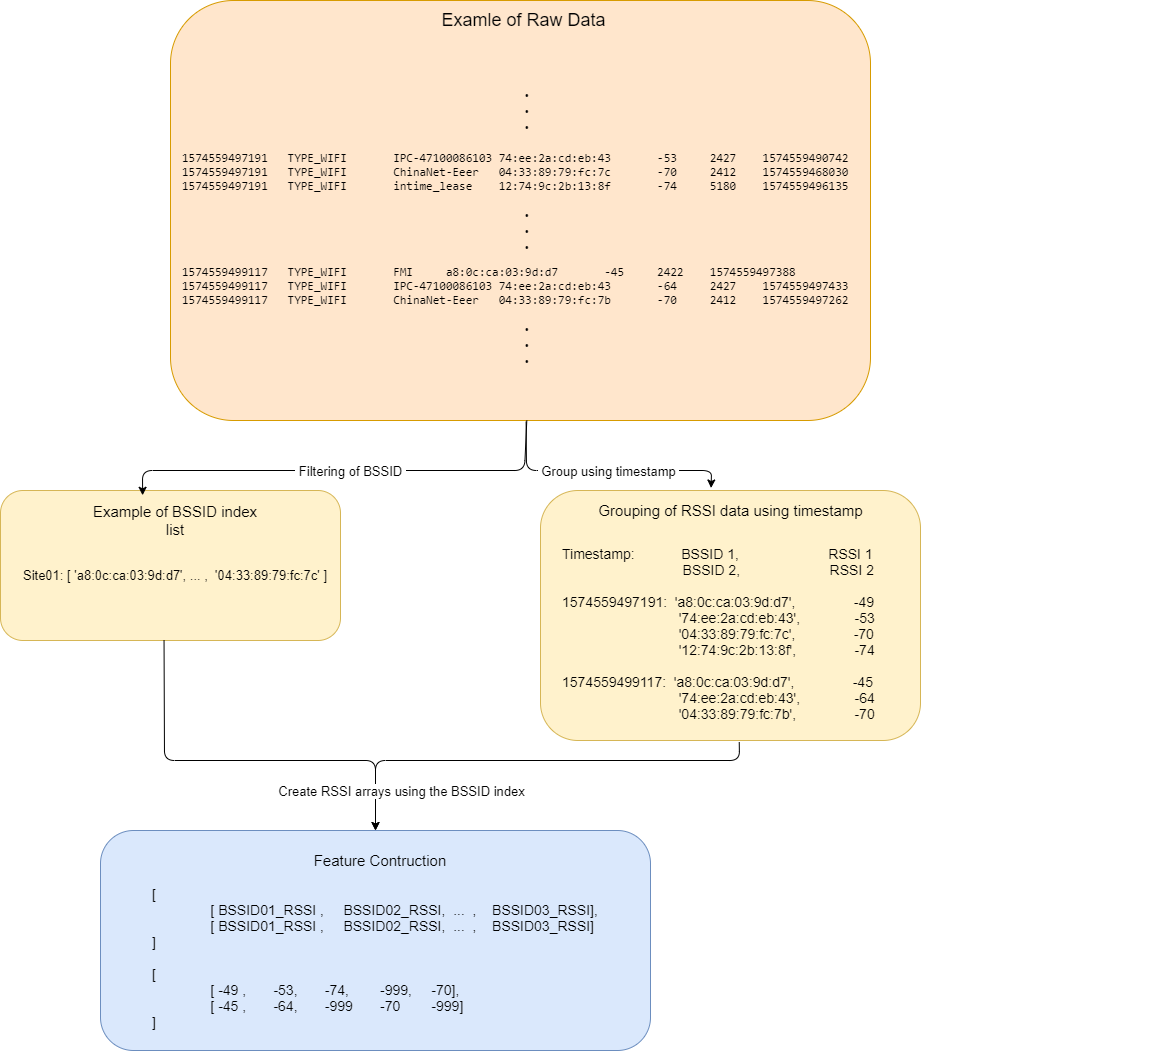
\includegraphics[width=1\textwidth]{Images/DataStandard/feat_eng_labeled (1).png}
    \caption{Labeled Dataset construction. The orange box shows a snippet of the raw dataset. }
    \label{fig:feat_labeled}
\end{figure}

As shown in \textbf{\autoref{alg:rssi}}, the feature engineering algorithm consists of a for-loop that will iterate all sites in the training data. This for-loop consists of two other for-loops, where the first will iterate through all the paths in a given site, and retrieve the relevant information. %It will hereafter append all the Wi-Fi measurements to a list, and all the waypoints to another list. 
The relevant information (\textit{wifi\_list}) will be grouped according to its timestamps, and these groups will be iterated through in the next for-loop on line 15, where the waypoint with the least difference between the group and each waypoint in the \textit{waypoints} list will be saved as the \textit{ground} result, which will be appended to the \textit{ground\_truth} list. The \gls{rssi} values from the group will be re-indexed and saved in \textit{feat}, which will be appended to the \textit{train\_data} list. As seen on line 21, the yield statement is used instead of a return statement. The yield statement indicates that we are working with a generator function. When working with a return statement, the statement would terminate the function entirely, whereas the yield statement will pause the function and save all of the states before continuing to successive calls.

\begin{algorithm}[H]
\SetAlgoLined
\SetKw{KwIn}{in}
\SetKwInOut{Input}{Input}
\Input{$\text{train\_data}$ which is organised into sites and further into paths}
\KwResult{($\text{site}_{x}$, $\text{train\_data}_{x}$, $\text{ground\_truth}_{x}$)}
 \For{$\text{site}_{x}$ \KwIn $\text{train\_data}$}{
  $\text{train\_data}_{x}$ = [], $\text{ground\_truth}_{x}$=[]\;
  Create $bssid\_index$ which is the set of BSSID values in the data for $\text{site}_{x}$\;
  \For{$\text{path}_{x}$ \KwIn $\text{site}_{x}$}{
    $wifi\_list$ = [], $waypoints$=[]\;
    \For{$measurement$ \KwIn $\text{path}_{x}$}{
        \If{$measurement$["type"]== $\text{TYPE\_WIFI}$}{
            $wifi\_list$.append($measurement$)\;
        }\ElseIf{$measurement$["type"]== $\text{waypoint}$}{
            $waypoints$.append($measurement$)
        }
    }
    Group $wifi\_list$ according to the timestamp into $grouped\_measmts$\;
    \For{$group$ \KwIn $grouped\_measmts$}{
        Calculate waypoint with least difference in timestamps between the $group$ and each waypoint in $waypoints$ and save the result as $ground$\;
        Take the RSSI-values from $group$ and reindex according to $bssid\_index$ and save in $feat$\;
        $\text{train\_data}_{x}$.append($feat$),$\text{ground\_truth}_{x}$.append($ground$)\;
    }
  }
  yield $\text{site}_{x}$,$\text{train\_data}_{x}$, $\text{ground\_truth}_{x}$\;
 }
 \caption{\gls{rssi}-labeling.}
 \label{alg:rssi}
\end{algorithm}

To create the features consisting of \gls{rssi} values, it is necessary to ensure that \gls{rssi} values are ordered such that the \textit{i}th value in a specific feature sample corresponds to data collected from one device (\gls{bssid}). This step is encapsulated by line 3 in \textbf{\autoref{alg:rssi}}. To this end, we use the \gls{bssid} values to uniquely distinguish the \gls{rssi} values from each other. Therefore, a pass over all data for a particular site is first made, where the \gls{bssid} values are collected to be used in the Feature Construction step in \textbf{\autoref{fig:feat_labeled}}. The \gls{bssid} values with less than a specific amount are then removed. This specific amount is set to 1000, but can be changed. The idea behind this filtering is that \gls{rssi} values with few occurrences will likely not contribute to the training of the models and might make it harder for the models to generalise. By performing this filtering, we observed that for approximately 5 \% of the features, all \gls{rssi} values were removed. To combat this, we include \gls{rssi} values from the test data when filtering. For the missing or unknown \gls{rssi} values, it will be set to -999 in the resulting feature. The result of collecting and filtering the \gls{bssid} values is shown \textit{Example of BSSID index} in \textbf{\autoref{fig:feat_labeled}}. 
The resulting \gls{bssid} set will be used as an index for the features. %To construct the features, a second pass over the data is made, where the measurement data is grouped by the timestamp. For each group, the \gls{rssi} values are extracted and an array is created by using the \gls{bssid} list and the \gls{rssi} values. For the \gls{bssid} indices with \gls{rssi} value in the group, the value will be set to -999.%The intuition behind this is to include a logarithmic activation function or a similar function to the input layer such that the values with -999 will have a small value. 

To gather multiple \gls{rssi} sensor measurements, we use the timestamp property in the measurements to group them together. This phase occurs in the right yellow box in \textbf{\autoref{fig:feat_labeled}}, and lines 14 to 19 in \textbf{\autoref{alg:rssi}}. The goal of location fingerprinting is to estimate the location given measurements at a certain time, making it reasonable to group with the timestamp. We will be using \gls{rssi} data, and this means that Wi-Fi and Bluetooth data can be used. As the Wi-Fi data is more prevalent in the dataset, we will be starting with this data. 
%After grouping the measurement data by the timestamp for each group, the \gls{rssi} values are extracted, and an feature sample is created by using a \gls{bssid} index for a site. For the \gls{bssid} indices without a \gls{rssi} value in the group, the value will be set to -999. To find the ground truth for each group, the temporally nearest waypoint to the group is found and treated as the ground truth along with the floor number which is specified in the file path to the data.

% \begin{wrapfigure}{r}{0.5\textwidth}
%   \begin{center}
%     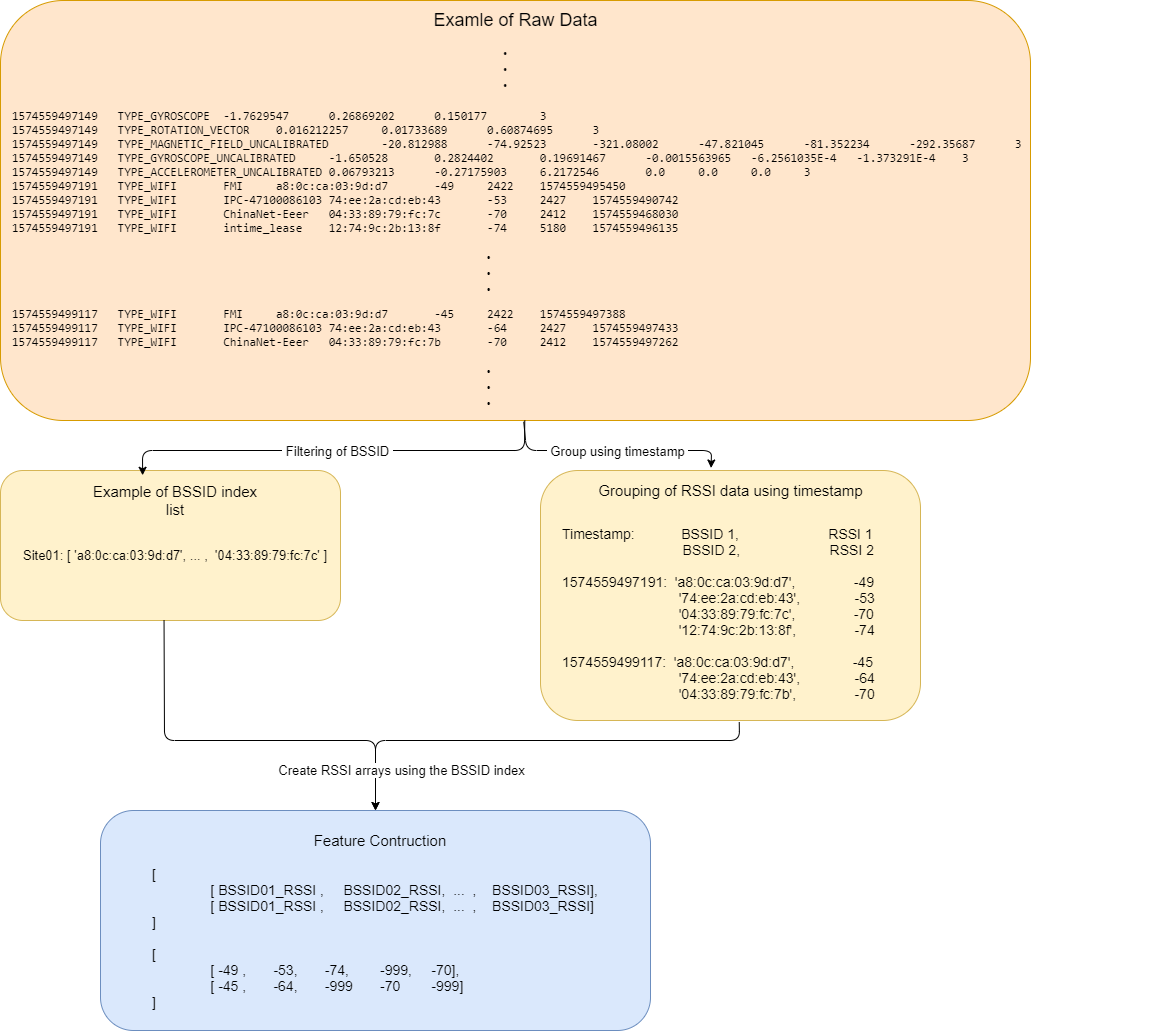
\includegraphics[width=0.48\textwidth]{Images/DataStandard/feat_eng_labeled.png}
%   \end{center}
%   \caption{Labeled Dataset Constuction}
% \end{wrapfigure}

\subsection{Time Series Data Formatting}

The time series dataset is similar to the RSSI-dataset other than the fact that the ordering of the measurements matter. 

Time-series data refers to a set of observations recorded over a given period of time at equally spaced time intervals. Time-series data is a type of sequence data, but in a time-series dataset, the observations are recorded based on timestamps. For instance, in a DNA sequence the order is important, but it is not ordered based on a timestamp \cite{Yalcın2021}. Time-series data gives us the opportunity to track changes over time, and in our case, the measurements given in the Kaggle dataset gives us the ability to track the movement of a device. 

This means that the feature samples should be organised into series, where each series contains a sequence of feature samples. These series should be organised into an list-based structure, and the corresponding ground truth data should be stored into another list-based structure, where \textit{i}th entry in feature series corresponds to the \textit{i}th entry in the ground truth series.

The algorithm for the time series labeling is very similar to the one presented in \textbf{\autoref{alg:rssi}}. The difference lies in line 5 and 21 in \textbf{\autoref{alg:time_series}}, where two new arrays are being created to hold the time series data, and afterwards appended to the training data and the ground truth data.

\begin{algorithm}[H]
\SetAlgoLined
\SetKw{KwIn}{in}
\SetKwInOut{Input}{Input}
\Input{$\text{train\_data}$ which is organised into sites and further into paths}
\KwResult{($\text{site}_{x}$, $\text{train\_data}_{x}$, $\text{ground\_truth}_{x}$)}

 \For{$\text{site}_{x}$ \KwIn $\text{train\_data}$}{
  $\text{train\_data}_{x}$ = [], $\text{ground\_truth}_{x}$=[]\;
  Create $bssid\_index$ which is the set of BSSID values in the data for $\text{site}_{x}$\;
  \For{$\text{path}_{x}$ \KwIn $\text{site}_{x}$}{
    $time\_series$ = [], $ts\_ground$=[]\;
    $wifi\_list$ = [], $waypoints$=[]\;
    \For{$measurement$ \KwIn $\text{path}_{x}$}{
        \If{$measurement$["type"]== $\text{TYPE\_WIFI}$}{
            $wifi\_list$.append($measurement$)\;
        }\ElseIf{$measurement$["type"]== $\text{waypoint}$}{
            $waypoints$.append($measurement$)
        }
    }
    Group $wifi\_list$ according to the timestamp into $grouped\_measmts$\;
    \For{$group$ \KwIn $grouped\_measmts$}{
        Calculate waypoint with least difference in timestamps between the $group$ and each waypoint in $waypoints$ and save the result as $ground$\;
        Take the RSSI-values from $group$ and reindex according to $bssid\_index$ and save in $feat$\;
        $time_series$.append($feat$),$ts_ground$.append($ground$)\;
    }
    $\text{train\_data}_{x}$.append($time\_series$),  $\text{ground\_truth}_{x}$.append($ts\_ground$)
  }
  yield $\text{site}_{x}$,$\text{train\_data}_{x}$, $\text{ground\_truth}_{x}$\;
 }
 \caption{Time Series labeling.}
 \label{alg:time_series}
\end{algorithm}
%https://online.stat.psu.edu/stat510/lesson/1/1.1



\subsection{Inertial Measurement Unit Dataset Creation}
The \gls{imu} dataset creation is for the \gls{imu}-based methods. The purpose of the formatting of the data for the \gls{imu}-based methods is purely for evaluating the methods as no learning is necessary for this type of indoor position estimation.
The basic idea with the feature engineering for the \gls{imu}-based methods is similar to the \gls{rssi}-based feature enginnering in that we once more group the \gls{imu} data according to timestamp. After the grouping, we will extract the relevant information into a list, which can then included as features.

\begin{algorithm}[H]
\SetAlgoLined
\SetKw{KwIn}{in}
\SetKwInOut{Input}{Input}
\Input{$\text{train\_data}$ which is organised into sites and further into paths}
\KwResult{($\text{path}_{x}$, $\text{train\_data}_{x}$, $\text{ground\_truth}_{x}$)}
 \For{$\text{site}_{x}$ \KwIn $\text{train\_data}$}{
  $\text{train\_data}_{x}$ = [], $\text{ground\_truth}_{x}$=[]\;
  \For{$\text{path}_{x}$ \KwIn $\text{site}_{x}$}{
    $imu\_list$ = [], $waypoints$=[]\;
    \For{$measurement$ \KwIn $\text{path}_{x}$}{
        \If{$measurement$["type"]== $\text{TYPE\_ACCELEROMETER}$}{
            $imu\_list$.append($measurement$)\;
        }\ElseIf{$measurement$["type"]== $\text{TYPE\_MAGNETIC\_FIELD}$}{
            $imu\_list$.append($measurement$)\;
        }\ElseIf{$measurement$["type"]== $\text{TYPE\_GYROSCOPE}$}{
            $imu\_list$.append($measurement$)\;
        }\ElseIf{$measurement$["type"]== $\text{waypoint}$}{
            $waypoints$.append($measurement$)
        }
    }
    Group $imu\_list$ according to the timestamp into $grouped\_measmts$\;
    \For{$group$ \KwIn $grouped\_measmts$}{
        Calculate waypoint with least difference in timestamps between the $group$ and each waypoint in $waypoints$ and save the result as $ground$\;
        $\text{train\_data}_{x}$.append($feat$),$\text{ground\_truth}_{x}$.append($ground$)\;
    }
  yield $\text{site}_{x}$,$\text{train\_data}_{x}$, $\text{ground\_truth}_{x}$\;  
  }
 }
 \caption{\gls{imu}-labeling.}
 \label{alg:imu}
\end{algorithm}


\subsection{Min-Max Normalisation} \label{sec:minmaxnormalisation}
Min-max normalisation scales features so that all features are equally significant. Although, the one disadvantage is that it handles feature outliers poorly.
Min-max normalisation is a data normalisation method described by \textbf{\autoref{eq:min_max_normalisation}}. Functions $min_A$ and $max_A$ compute the minimum and maximum value of an attribute, $A$, respectively. Given a value $v_i$ of an attribute $A$ as input, min-max normalisation computes value $v_{i}'$ in the range $[new\_min_A, new\_max_A]$.\cite{Han_Kamber_2012}

\begin{equation}
    v_{i}' = \frac{v_i - min_A}{max_A - min_A} (new\_max_A - new\_min_A) + new\_min_A
    \label{eq:min_max_normalisation}
\end{equation}